% Kyle Geyser
% 12/2/12

\documentclass{beamer}
\usefonttheme[onlymath]{serif}
\useoutertheme{shadow}
\usecolortheme{seahorse}
\usepackage{amsmath, amsfonts, amssymb, amsthm}
\usepackage{graphicx}
\usepackage{movie15}
\usepackage{hyperref}

\def\e{\text{e}}
\def\L{\mathcal{L}}

\begin{document}
	
	\title{Solving parabolic PDEs in parallel via time discretization using Laplace transforms}
	\author{Kyle Geyser and Dylan Denning}
	\date{December 3, 2012}

	\frame{\titlepage} 
	
	\frame{\frametitle{The Problem}
		$$u_t+Au=f(t),\hspace{4mm}\text{for }t>0,\hspace{4mm}\text{with }u(0)=u_0$$ \\\vspace{1cm}
		where $A$ is the second-order differential operator ($\nabla^2$) \\
		and $u_0$ and $f(t)$ are given. \\\vspace{1cm}
		i.e. The heat equation...
	}
	
	\frame{\frametitle{The Transformed Problem}
		$$(zI+A)w(z)=u_0+\hat{f}(z)$$ \\\vspace{1cm}
		where $z$ is the transform variable, $I$ is the identity matrix, $\hat{f}(z)=\L\{f\}$, and $w(z)=\L\{u\}$. \\\vspace{1cm}
		Note: all functions above have implied spatial terms based on the dimensionality of the problem
	}
	
	\frame{\frametitle{The Solution: space}
		We find an approximation for $w(z)$ using the finite difference method with $m-1$ interior points, $m$ a chosen parameter.
		In one spacial dimension, $A$ is the $m-1\times m-1$ discrete Laplacian given by:
		$$A=\begin{bmatrix}
		2 & -1 & 0 & 0 & \cdots & \cdots & \cdots\\
		-1 & 2 & -1 & 0 & 0 & \cdots & \cdots \\
		0 & -1 & 2 & -1 & 0 & 0 & \cdots \\
		\vdots & & & \ddots & & & \vdots \\
		\vdots & & & & \ddots & & \vdots \\
		0 & 0 & \cdots & \cdots & -1 & 2 & -1 \\
		0 & 0 & \cdots & \cdots &\cdots & -1 & 2
		\end{bmatrix}$$
	}
	
	\small\frame{\frametitle{The Solution: space (continued)}
		The tridiagonal system we solve becomes
		$$\frac{1}{h^2}(zI+A)w(z)=g(t)$$
		where
		$$g(t)=\vec{u_0}+\vec{\hat{f}}(z)+\frac{1}{h^2}
		\begin{bmatrix}
			\alpha \\
			0 \\
			0 \\
			\vdots \\
			\beta
		\end{bmatrix}$$ \\
		with
		$$h=\frac{b-a}{m},\; a\text{ and } b\text{ the endpoints of our domain},\;\alpha=u(a),\;\beta=u(b),$$
		and
		$\vec{u_0}+\vec{\hat{f}}(z)$ vectors of size $m-1$ containing $u_0$ and $\hat{f}(z)$ evaluated at $x_i=a+ih,\hspace{4mm}i=1,2,...,m-1$.
	}
	
	\normalsize\frame{\frametitle{The Solution: time}
		Using a trapezoidal rule: \\
		$$u(t)\approx U_{N,\tau}(t)=2\text{Re}\left(\frac{1}{N\tau}\sum_{j=0}^{N-1}{}^\prime \tilde{\mu_j}\e^{z_jt}w(z_j)\right)$$ \\\vspace{1cm}
		where $z_j$ are the qudrature points on the transformed contour, \\
		$\tilde{\mu_j}$ are the weights associated with each $z_j$, \\
		$\tau$ is a time scaling parameter, \\
		and the ${}^\prime$ denotes halving the first term in the sum. \\\vspace{1cm}
		The first term is halved and the sum from $0$ to $N-1$ is doubled because of the even symmetry of the contour.
	}
	
	\frame{\frametitle{Parallel Approach}
		We parallelized the sum from the previous slide using MPI. \\\vspace{3mm}
		Using this approach, each core, except the first and last cores, computes a local sum corresponding to $\frac{N-1}{P}$ quadrature points. \\\vspace{3mm}
		The first core computes the first term in the full sum, and adds to that a local sum corresponding to $\frac{N-1}{P}$ quadrature points. \\\vspace{3mm}
		The last core computes a local sum corresponding to $\frac{N-1}{P}+\text{Mod}(N-1, P)$ quadrature points. \\\vspace{3mm}
		We then use \texttt{MPI\_Reduce} with the \texttt{master} core to reduce the local sums into a full sum.
	}
	
	\frame{\frametitle{Test PDE}
		$$u_t-u_{xx}=f(x,t),\hspace{4mm}\text{for }0<x<\pi,\;t>0,$$
		$$u(x,t)=0\hspace{4mm}\text{for }x=0\text{ and }\pi,\;t>0,$$
		with
		$$u(x,0)=u_0(x),\hspace{4mm}\text{for }0<x<\pi$$
		and
		$$f(x,t)=\e^{-t}\sin(x)+\e^{-2t}(2cos(t)-\sin(t))\sin(2x),$$
		$$u_0(x)=\sin(x)+\sin(2x),$$
 		$$\hat{f}(x,z)=\frac{1}{1+z}\sin(x)+\frac{2z+3}{(z+2)^2+1}\sin(2x)$$
	}
	
	\frame{\frametitle{Actual Solution}
		$$u(x,t)=(1+t)\e^{-t}\sin(x)+\cos(t)\e^{-2t}\sin(2x)$$
		\begin{figure}
			\movie[mouse, repeat]{animation.mpg}{ProjectFiles/results/movies/animation.mpg}
		\end{figure}
	}
	
	\frame{\frametitle{Results}
		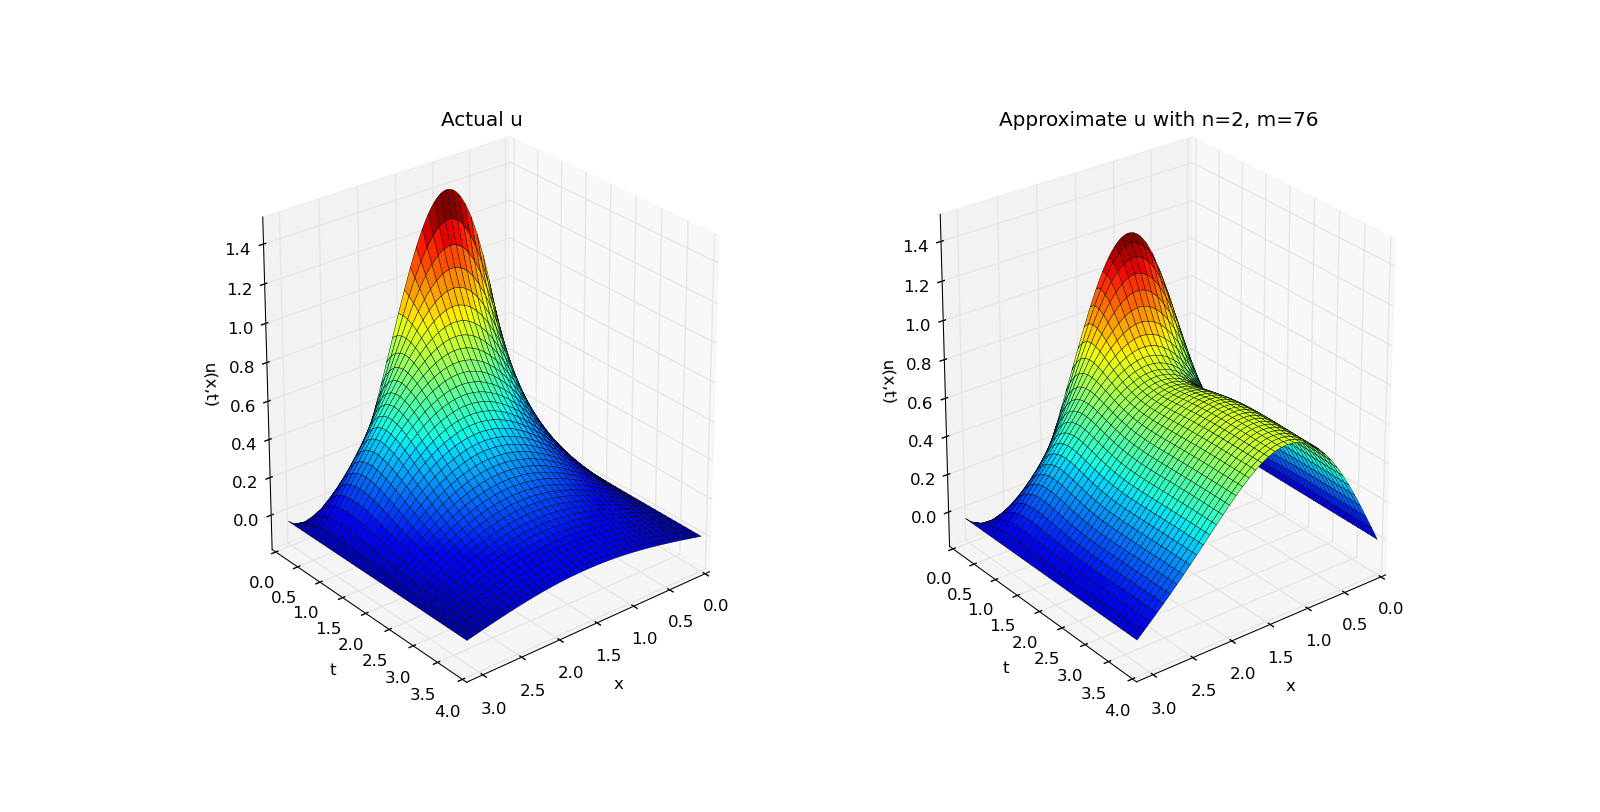
\includegraphics[trim = 6.5cm 3cm 6cm 2cm, width=\linewidth]{ProjectFiles/results/plots/n2m76.png}
	}
	
	\frame{\frametitle{Results}
		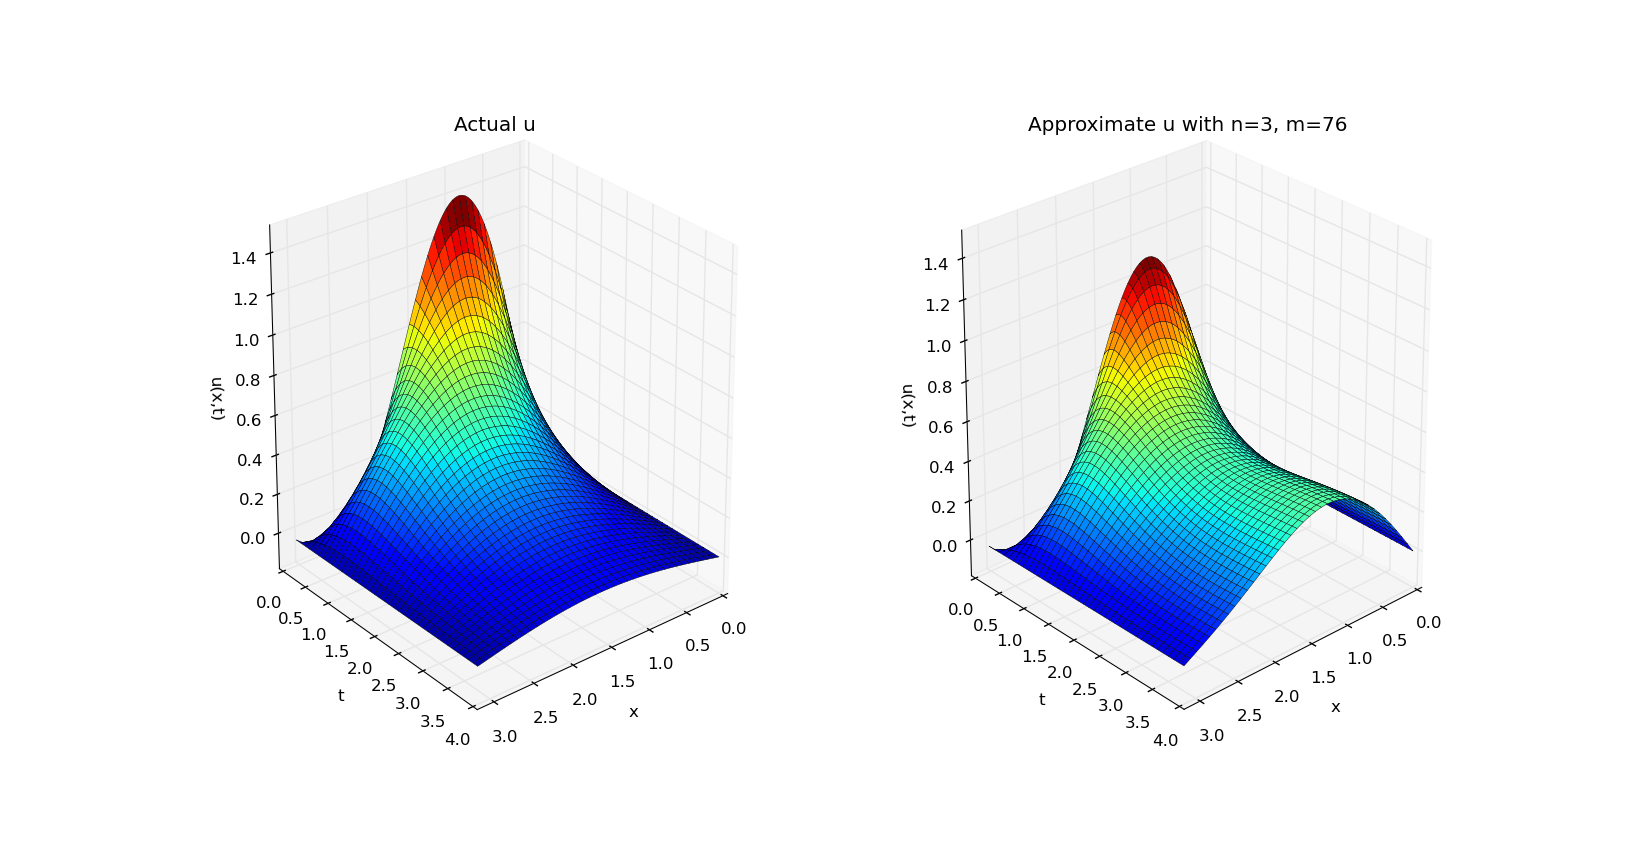
\includegraphics[trim = 6.5cm 3cm 6cm 2cm, width=\linewidth]{ProjectFiles/results/plots/n3m76.png}
	}
	
	\frame{\frametitle{Results}
		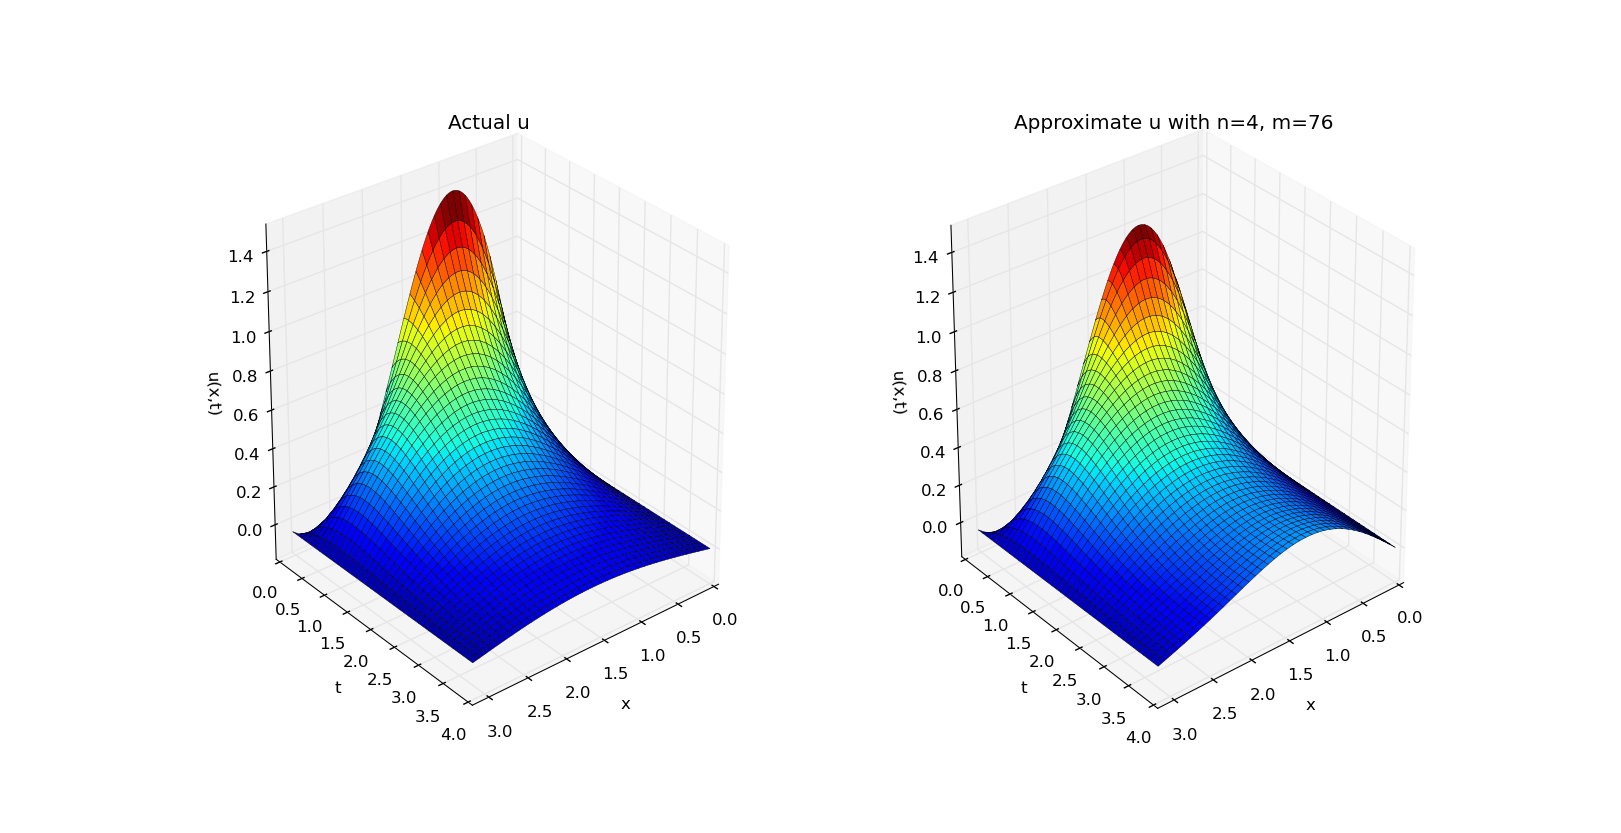
\includegraphics[trim = 6.5cm 3cm 6cm 2cm, width=\linewidth]{ProjectFiles/results/plots/n4m76.png}
	}
	
	\frame{\frametitle{Results}
		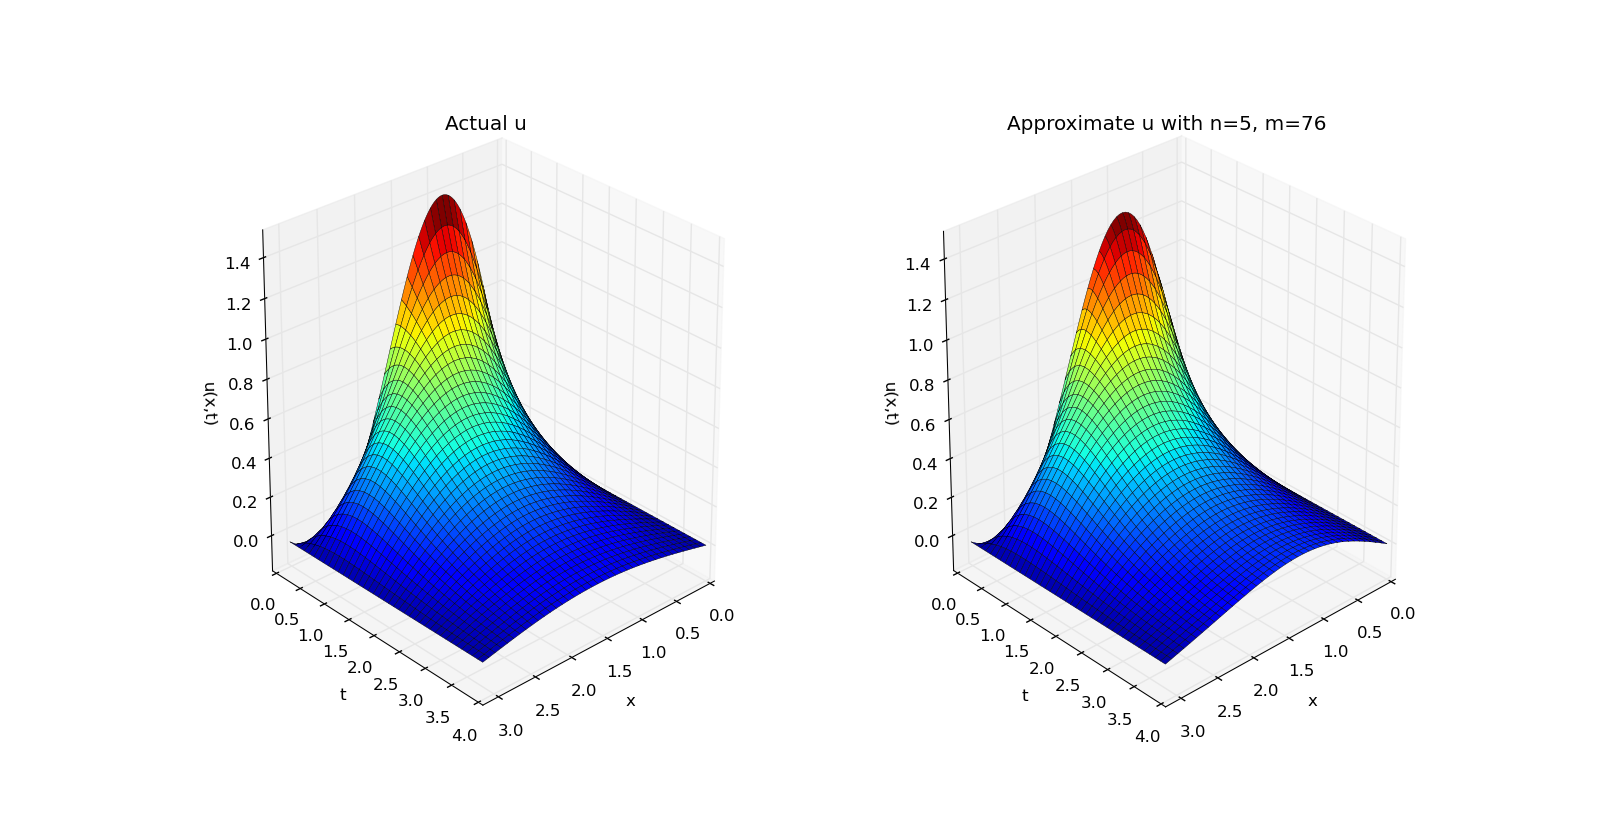
\includegraphics[trim = 6.5cm 3cm 6cm 2cm, width=\linewidth]{ProjectFiles/results/plots/n5m76.png}
	}
	
	\frame{\frametitle{Results}
		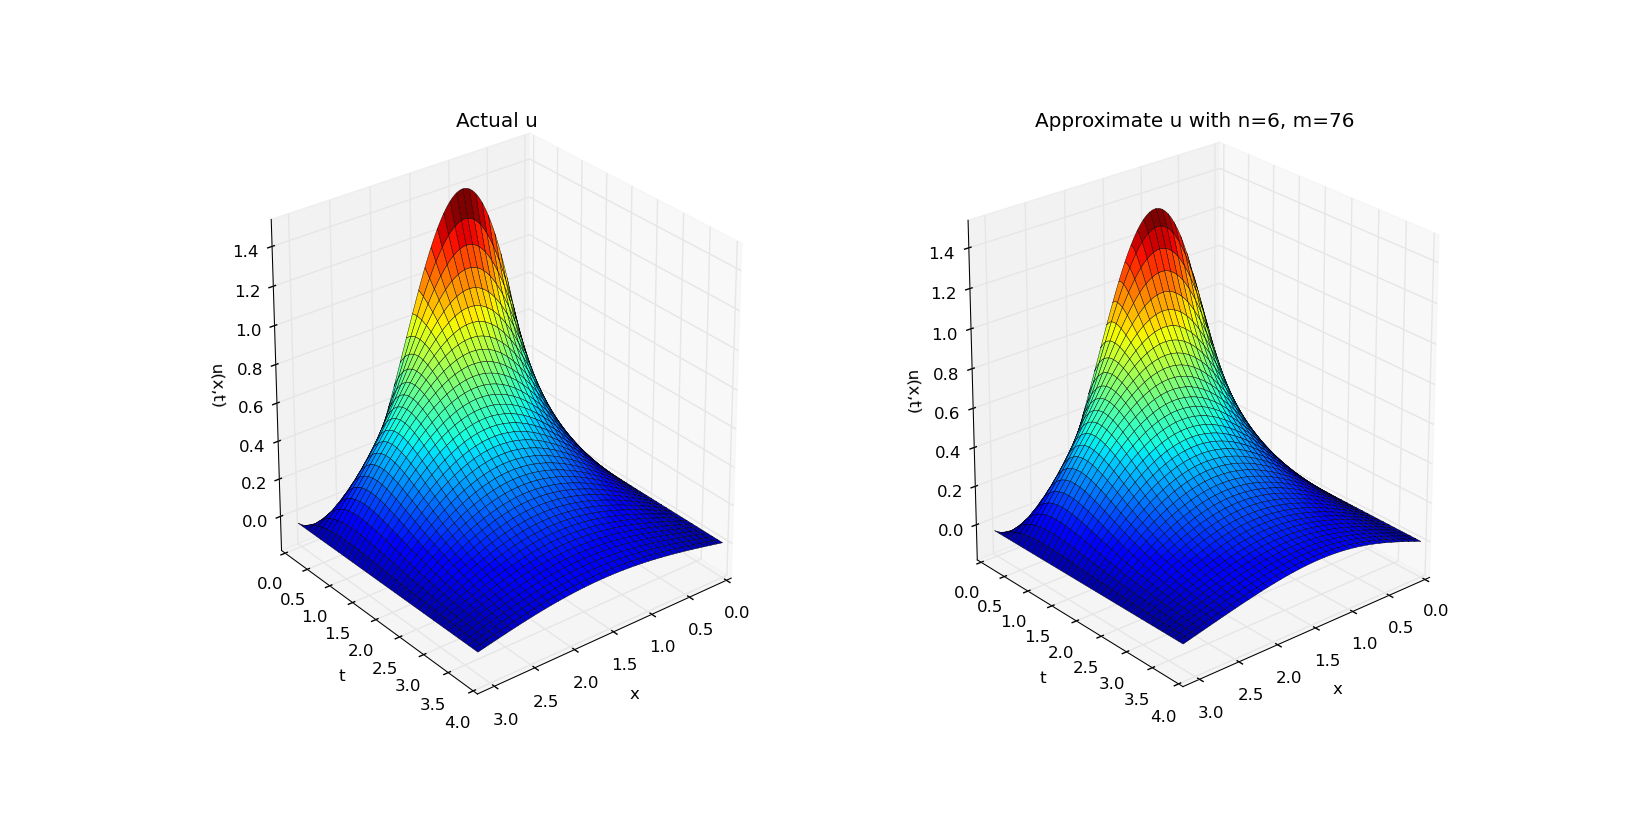
\includegraphics[trim = 6.5cm 3cm 6cm 2cm, width=\linewidth]{ProjectFiles/results/plots/n6m76.png}
	}
	
	\frame{\frametitle{Results}
		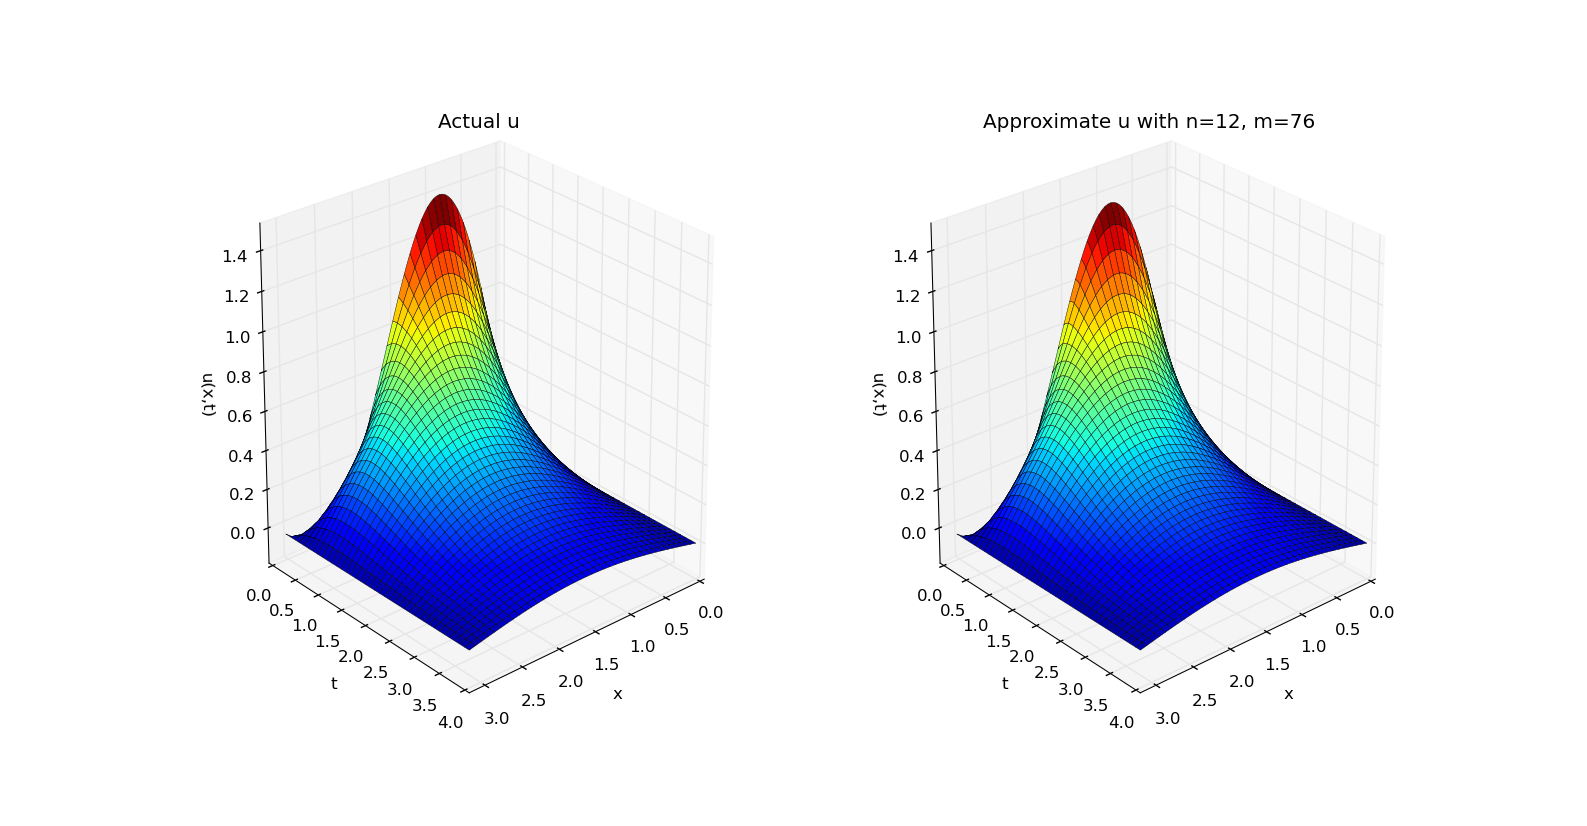
\includegraphics[trim = 6.5cm 3cm 6cm 2cm, width=\linewidth]{ProjectFiles/results/plots/n12m76.png}
	}
	
	\frame{\frametitle{Results}
		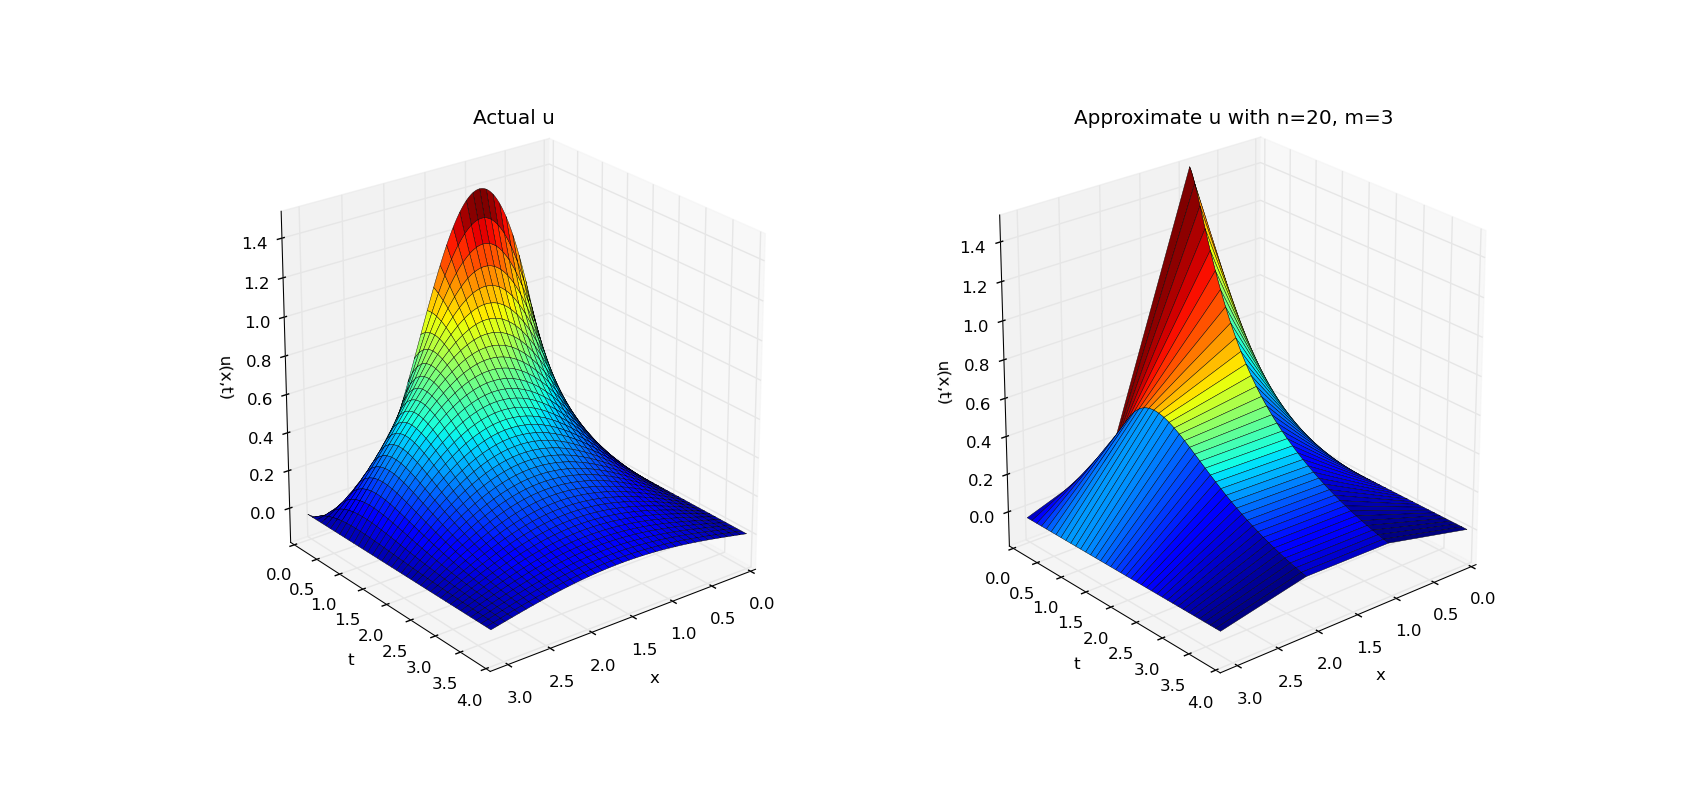
\includegraphics[trim = 6.5cm 3cm 6cm 2cm, width=\linewidth]{ProjectFiles/results/plots/n20m3.png}
	}
	
	\frame{\frametitle{Results}
		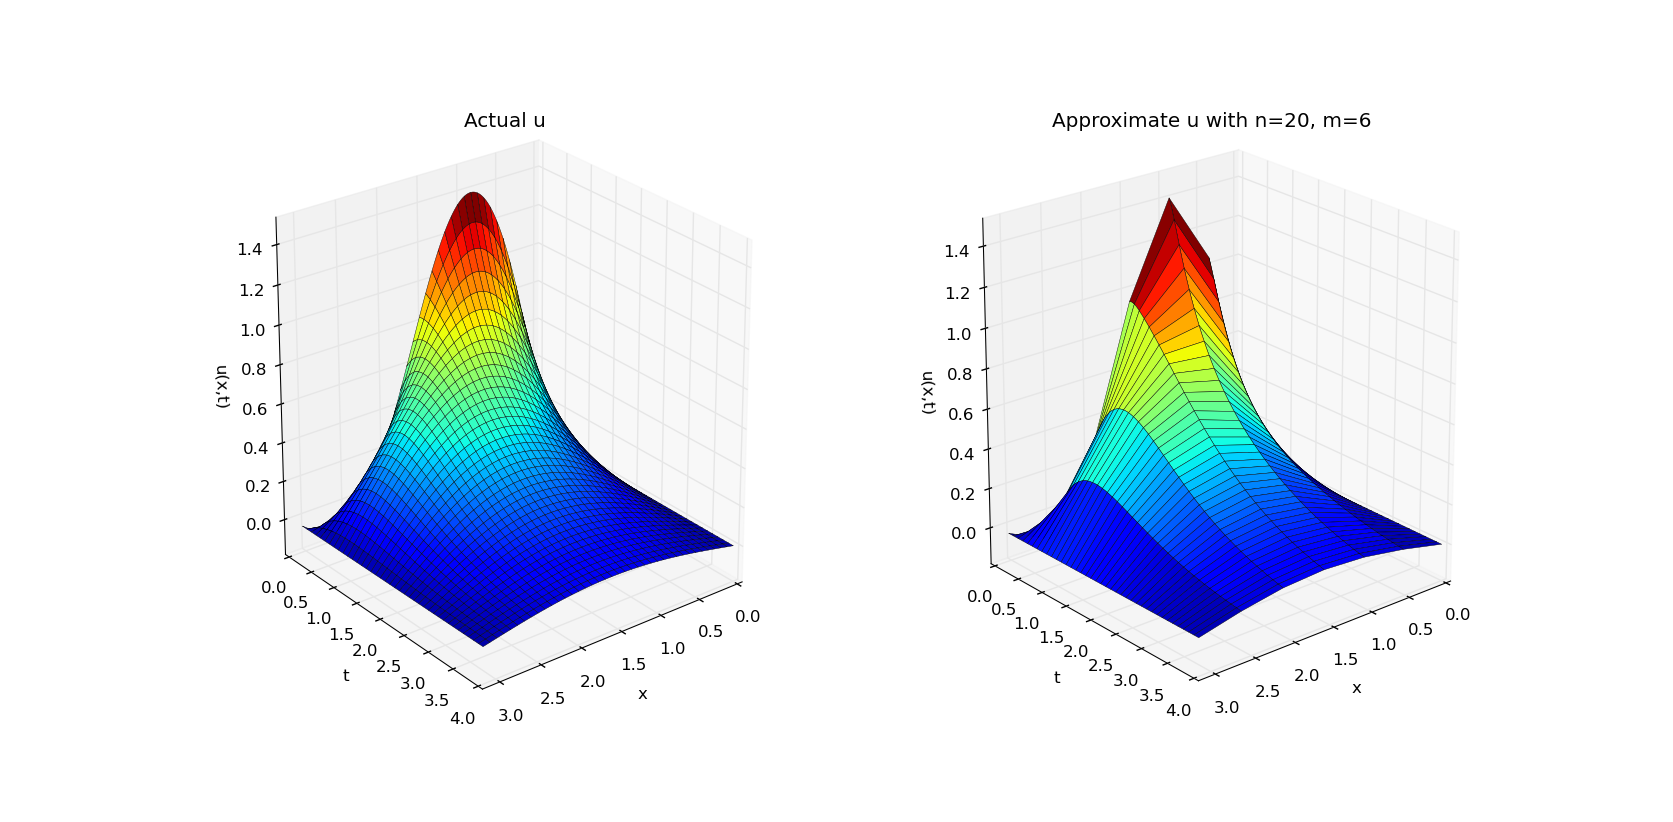
\includegraphics[trim = 6.5cm 3cm 6cm 2cm, width=\linewidth]{ProjectFiles/results/plots/n20m6.png}
	}
	
	\frame{\frametitle{Results}
		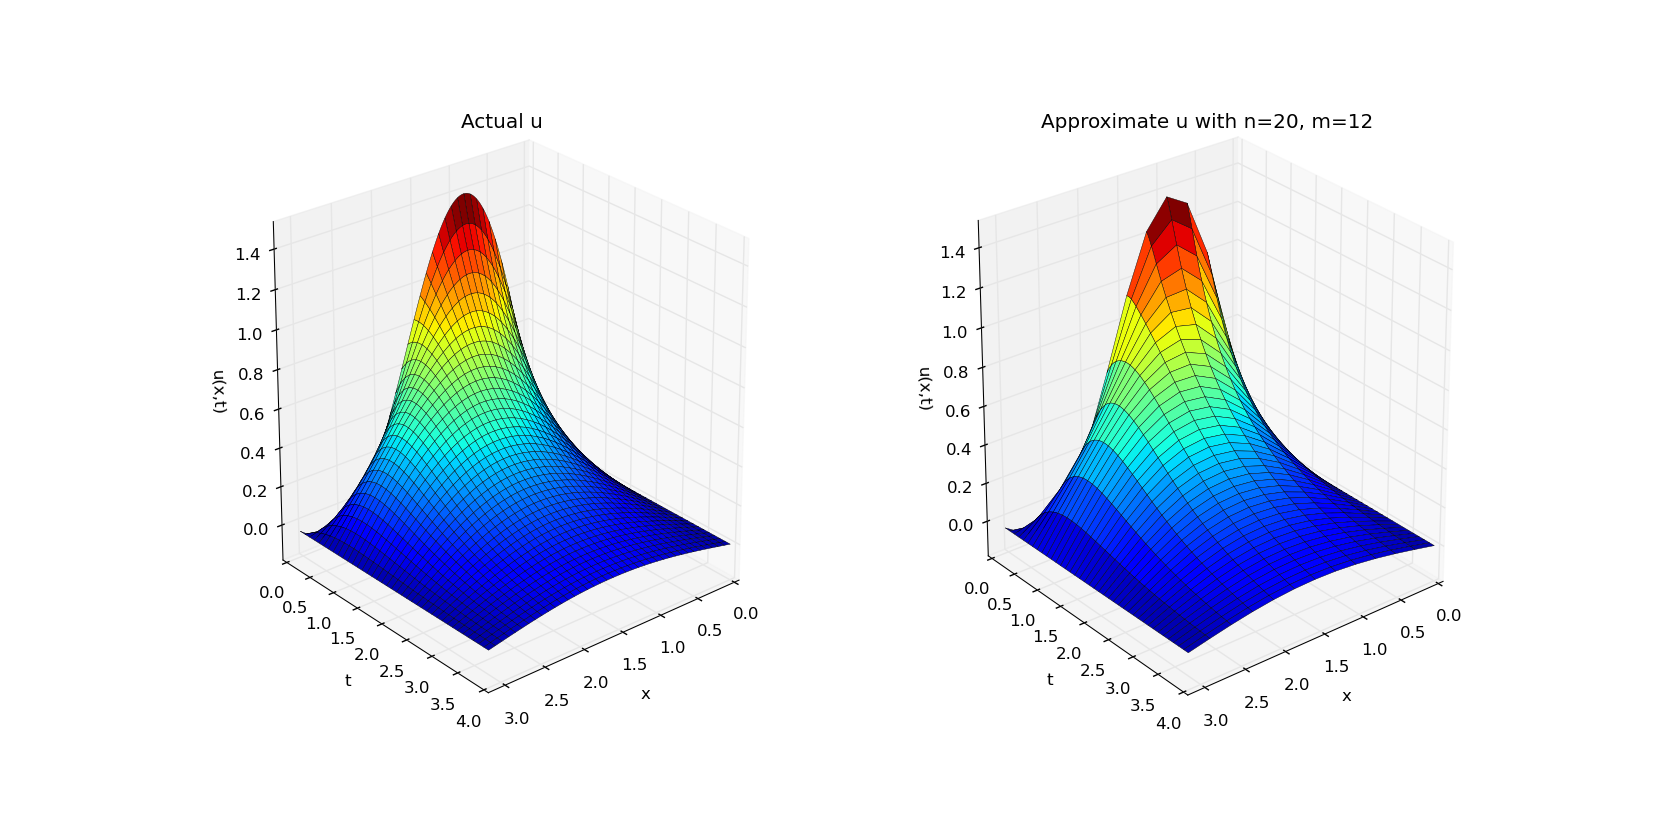
\includegraphics[trim = 6.5cm 3cm 6cm 2cm, width=\linewidth]{ProjectFiles/results/plots/n20m12.png}
	}
	
	\frame{\frametitle{Results}
		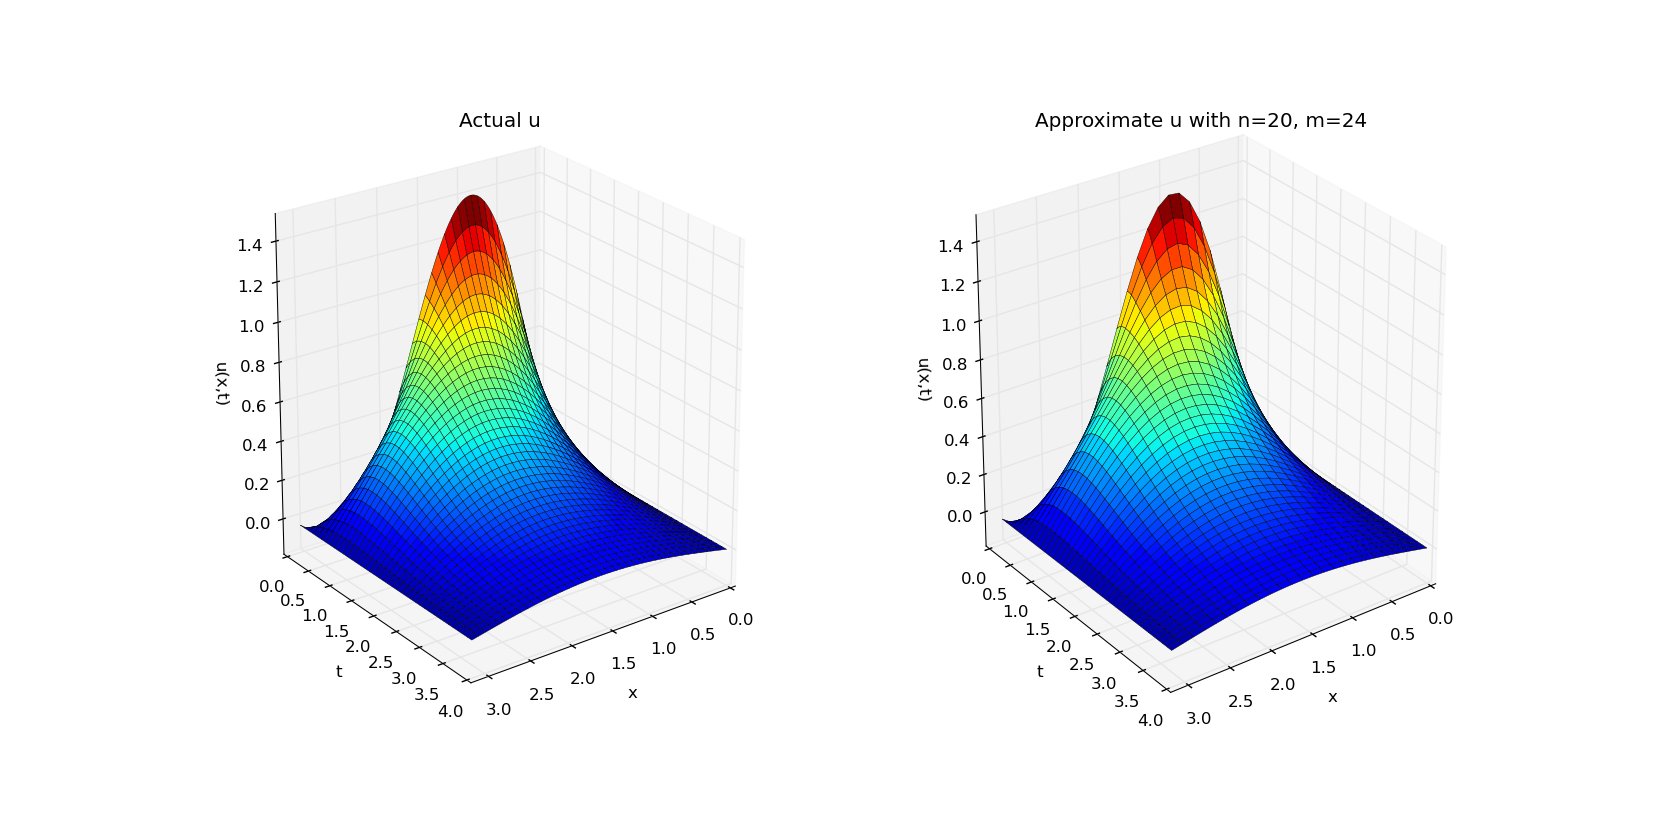
\includegraphics[trim = 6.5cm 3cm 6cm 2cm, width=\linewidth]{ProjectFiles/results/plots/n20m24.png}
	}
	
	\frame{\frametitle{Results}
		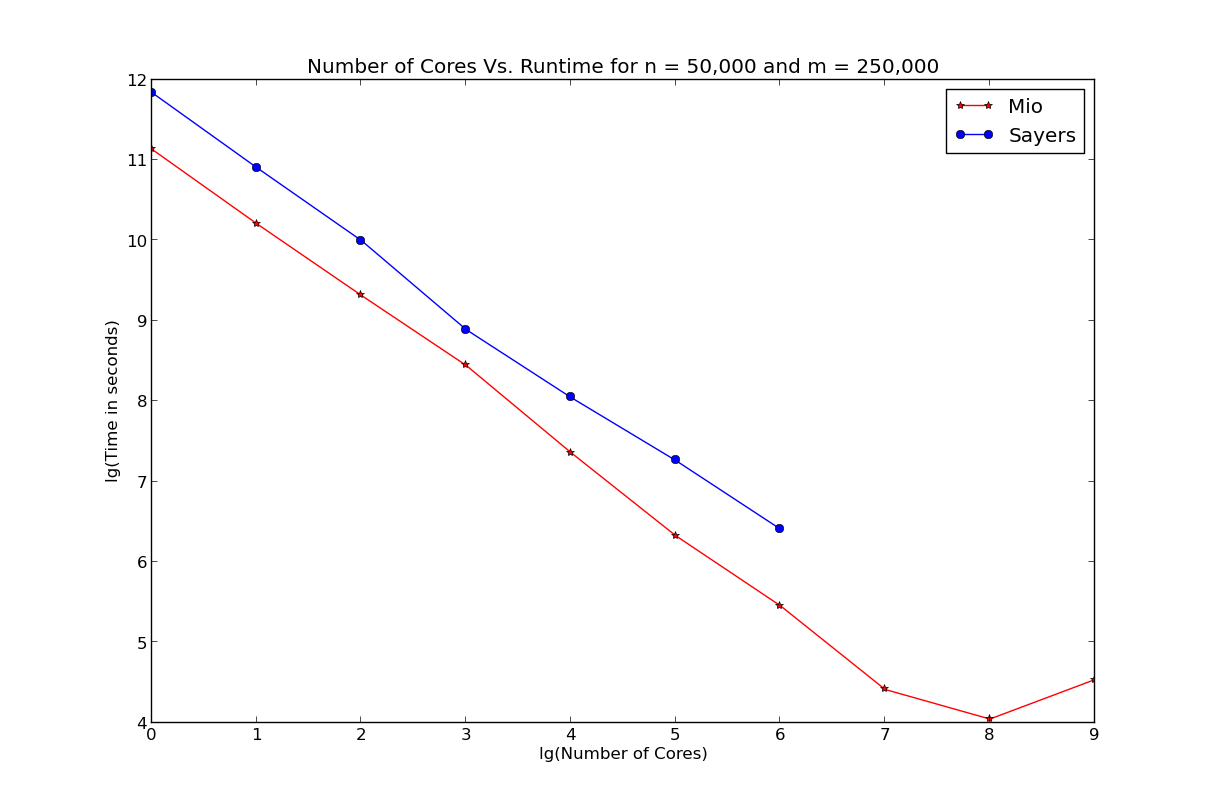
\includegraphics[width=\linewidth]{ProjectFiles/results/plots/coresVtime.png}
	}
	
	\frame{\frametitle{Results}
		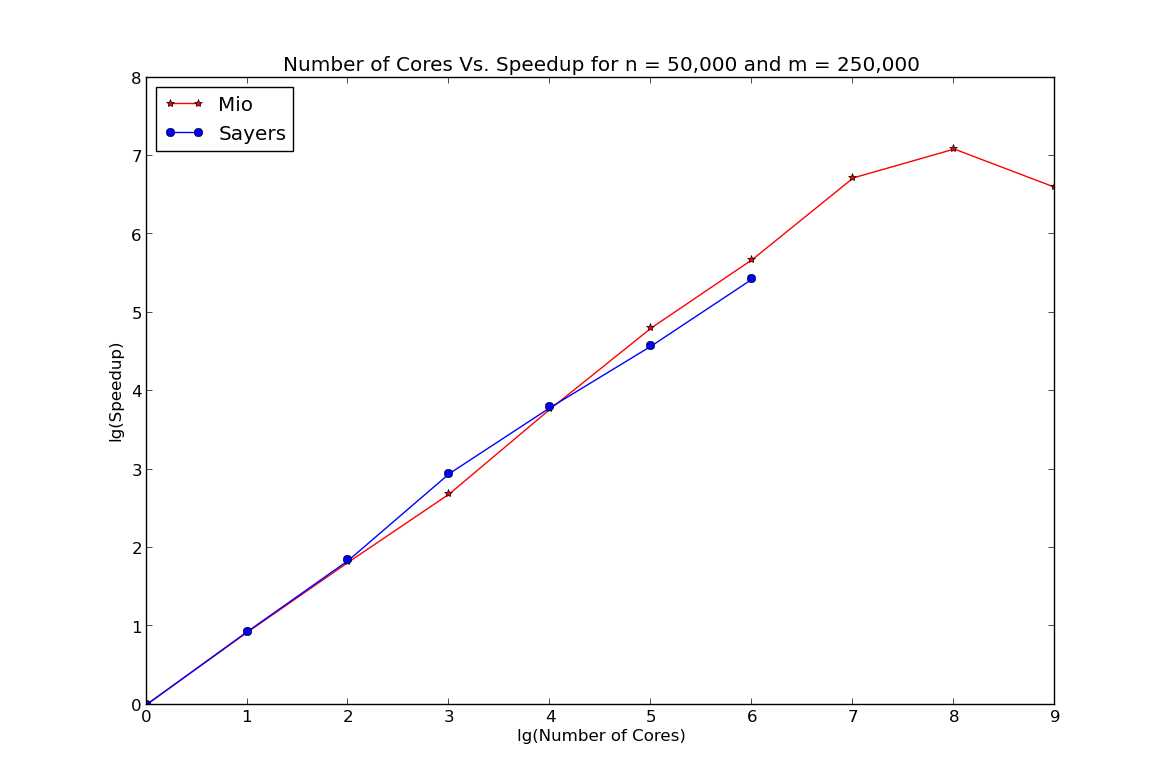
\includegraphics[width=\linewidth]{ProjectFiles/results/plots/coresVspeedup.png}
	}
	
	\frame{\frametitle{Results}
		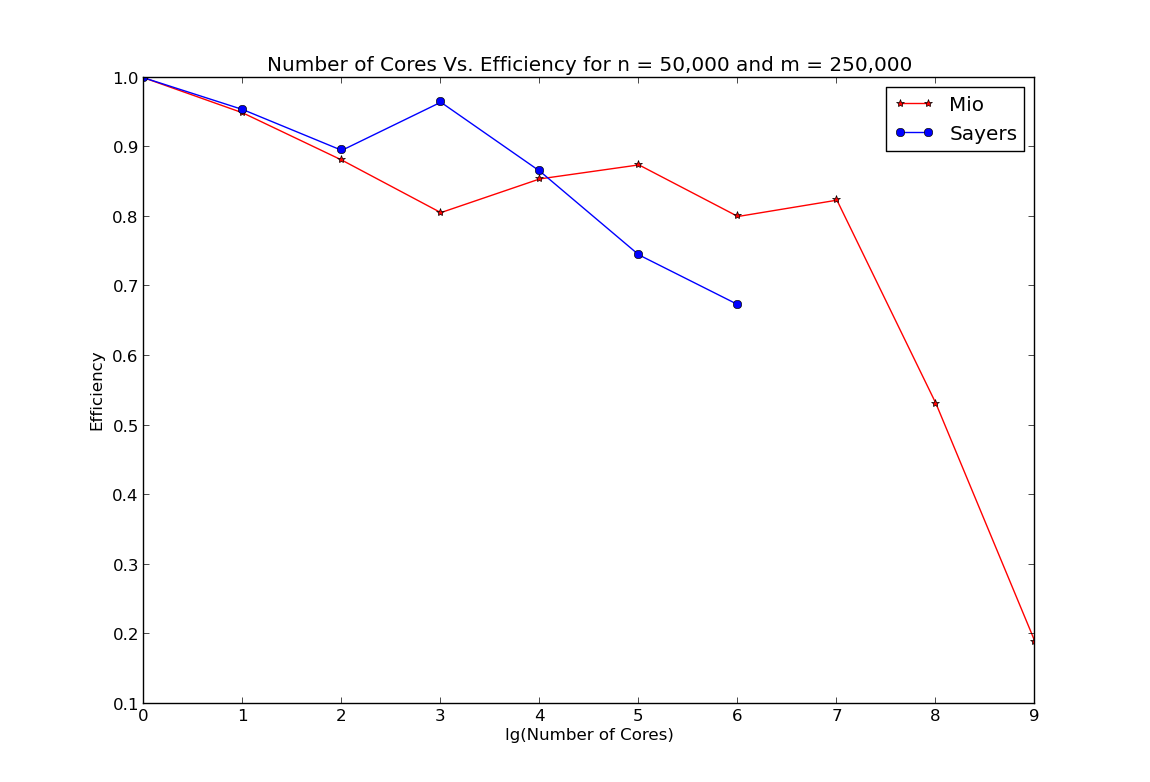
\includegraphics[width=\linewidth]{ProjectFiles/results/plots/coresVefficiency.png}
	}
	
	\frame{\frametitle{Results}
		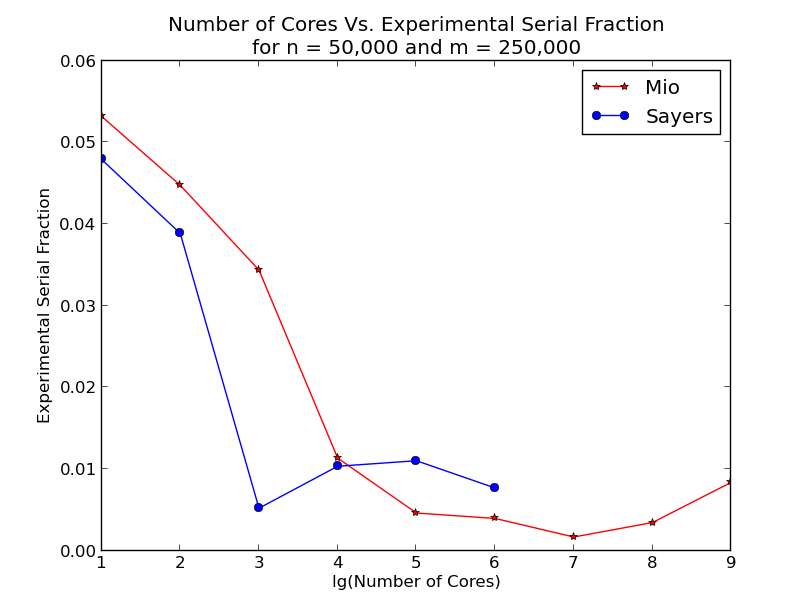
\includegraphics[width=\linewidth]{ProjectFiles/results/plots/coresVexpserialfrac.png}
	}
	
	\frame{\frametitle{References}
		Dongwoo Sheen, Ian H. Sloan, and Vidar Thom\'{e}e,
			\emph{A parallel method for time discretization of parabolic equations based on Laplace transformation and quadrature}.
			IMA Journal of Numerical Analysis (2003) 23,
			269-299 \\\vspace{1cm}
			
		Mahadevan Ganesh, PhD, Colorado School of Mines
	}
	
\end{document}
